% Created by tikzDevice version 0.10.1 on 2018-01-15 11:46:44
% !TEX encoding = UTF-8 Unicode
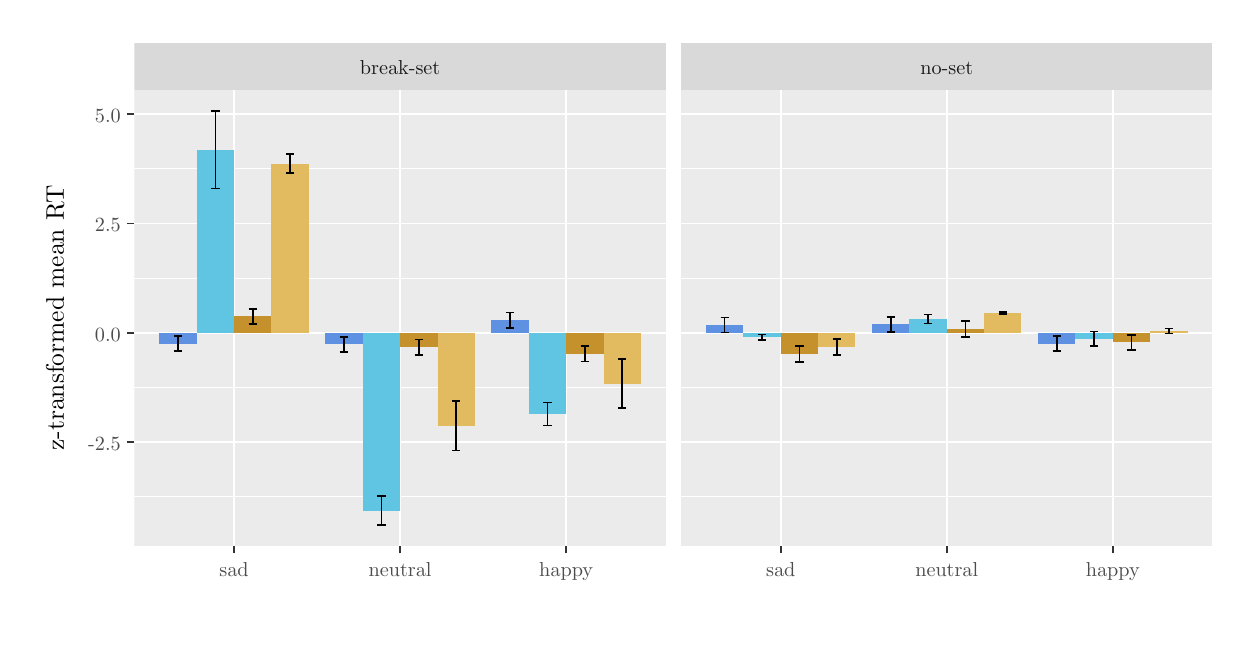
\begin{tikzpicture}[x=1pt,y=1pt]
\definecolor{fillColor}{RGB}{255,255,255}
\path[use as bounding box,fill=fillColor,fill opacity=0.00] (0,0) rectangle (433.62,216.81);
\begin{scope}
\path[clip] (  0.00,  0.00) rectangle (433.62,216.81);
\definecolor{drawColor}{RGB}{255,255,255}
\definecolor{fillColor}{RGB}{255,255,255}

\path[draw=drawColor,line width= 0.6pt,line join=round,line cap=round,fill=fillColor] ( -0.00,  0.00) rectangle (433.62,216.81);
\end{scope}
\begin{scope}
\path[clip] ( 38.57, 29.59) rectangle (230.60,194.25);
\definecolor{fillColor}{gray}{0.92}

\path[fill=fillColor] ( 38.57, 29.59) rectangle (230.60,194.25);
\definecolor{drawColor}{RGB}{255,255,255}

\path[draw=drawColor,line width= 0.3pt,line join=round] ( 38.57, 47.34) --
	(230.60, 47.34);

\path[draw=drawColor,line width= 0.3pt,line join=round] ( 38.57, 86.83) --
	(230.60, 86.83);

\path[draw=drawColor,line width= 0.3pt,line join=round] ( 38.57,126.33) --
	(230.60,126.33);

\path[draw=drawColor,line width= 0.3pt,line join=round] ( 38.57,165.83) --
	(230.60,165.83);

\path[draw=drawColor,line width= 0.6pt,line join=round] ( 38.57, 67.08) --
	(230.60, 67.08);

\path[draw=drawColor,line width= 0.6pt,line join=round] ( 38.57,106.58) --
	(230.60,106.58);

\path[draw=drawColor,line width= 0.6pt,line join=round] ( 38.57,146.08) --
	(230.60,146.08);

\path[draw=drawColor,line width= 0.6pt,line join=round] ( 38.57,185.58) --
	(230.60,185.58);

\path[draw=drawColor,line width= 0.6pt,line join=round] ( 74.58, 29.59) --
	( 74.58,194.25);

\path[draw=drawColor,line width= 0.6pt,line join=round] (134.58, 29.59) --
	(134.58,194.25);

\path[draw=drawColor,line width= 0.6pt,line join=round] (194.59, 29.59) --
	(194.59,194.25);
\definecolor{fillColor}{RGB}{226,186,95}

\path[fill=fillColor] ( 88.08,106.58) rectangle (101.58,167.72);
\definecolor{fillColor}{RGB}{196,145,45}

\path[fill=fillColor] ( 74.58,106.58) rectangle ( 88.08,112.45);
\definecolor{fillColor}{RGB}{95,197,226}

\path[fill=fillColor] ( 61.07,106.58) rectangle ( 74.58,172.73);
\definecolor{fillColor}{RGB}{95,145,226}

\path[fill=fillColor] ( 47.57,102.60) rectangle ( 61.07,106.58);
\definecolor{fillColor}{RGB}{226,186,95}

\path[fill=fillColor] (148.09, 72.95) rectangle (161.59,106.58);
\definecolor{fillColor}{RGB}{196,145,45}

\path[fill=fillColor] (134.58,101.37) rectangle (148.09,106.58);
\definecolor{fillColor}{RGB}{95,197,226}

\path[fill=fillColor] (121.08, 42.30) rectangle (134.58,106.58);
\definecolor{fillColor}{RGB}{95,145,226}

\path[fill=fillColor] (107.58,102.42) rectangle (121.08,106.58);
\definecolor{fillColor}{RGB}{226,186,95}

\path[fill=fillColor] (208.09, 88.15) rectangle (221.59,106.58);
\definecolor{fillColor}{RGB}{196,145,45}

\path[fill=fillColor] (194.59, 98.97) rectangle (208.09,106.58);
\definecolor{fillColor}{RGB}{95,197,226}

\path[fill=fillColor] (181.09, 77.23) rectangle (194.59,106.58);
\definecolor{fillColor}{RGB}{95,145,226}

\path[fill=fillColor] (167.59,106.58) rectangle (181.09,111.12);
\definecolor{drawColor}{RGB}{0,0,0}

\path[draw=drawColor,line width= 0.6pt,line join=round] ( 93.33,171.22) --
	( 96.33,171.22);

\path[draw=drawColor,line width= 0.6pt,line join=round] ( 94.83,171.22) --
	( 94.83,164.23);

\path[draw=drawColor,line width= 0.6pt,line join=round] ( 93.33,164.23) --
	( 96.33,164.23);

\path[draw=drawColor,line width= 0.6pt,line join=round] ( 79.83,115.25) --
	( 82.83,115.25);

\path[draw=drawColor,line width= 0.6pt,line join=round] ( 81.33,115.25) --
	( 81.33,109.64);

\path[draw=drawColor,line width= 0.6pt,line join=round] ( 79.83,109.64) --
	( 82.83,109.64);

\path[draw=drawColor,line width= 0.6pt,line join=round] ( 66.32,186.76) --
	( 69.33,186.76);

\path[draw=drawColor,line width= 0.6pt,line join=round] ( 67.82,186.76) --
	( 67.82,158.70);

\path[draw=drawColor,line width= 0.6pt,line join=round] ( 66.32,158.70) --
	( 69.33,158.70);

\path[draw=drawColor,line width= 0.6pt,line join=round] ( 52.82,105.30) --
	( 55.82,105.30);

\path[draw=drawColor,line width= 0.6pt,line join=round] ( 54.32,105.30) --
	( 54.32, 99.91);

\path[draw=drawColor,line width= 0.6pt,line join=round] ( 52.82, 99.91) --
	( 55.82, 99.91);

\path[draw=drawColor,line width= 0.6pt,line join=round] (153.34, 81.92) --
	(156.34, 81.92);

\path[draw=drawColor,line width= 0.6pt,line join=round] (154.84, 81.92) --
	(154.84, 63.97);

\path[draw=drawColor,line width= 0.6pt,line join=round] (153.34, 63.97) --
	(156.34, 63.97);

\path[draw=drawColor,line width= 0.6pt,line join=round] (139.83,104.16) --
	(142.83,104.16);

\path[draw=drawColor,line width= 0.6pt,line join=round] (141.33,104.16) --
	(141.33, 98.57);

\path[draw=drawColor,line width= 0.6pt,line join=round] (139.83, 98.57) --
	(142.83, 98.57);

\path[draw=drawColor,line width= 0.6pt,line join=round] (126.33, 47.53) --
	(129.33, 47.53);

\path[draw=drawColor,line width= 0.6pt,line join=round] (127.83, 47.53) --
	(127.83, 37.07);

\path[draw=drawColor,line width= 0.6pt,line join=round] (126.33, 37.07) --
	(129.33, 37.07);

\path[draw=drawColor,line width= 0.6pt,line join=round] (112.83,105.12) --
	(115.83,105.12);

\path[draw=drawColor,line width= 0.6pt,line join=round] (114.33,105.12) --
	(114.33, 99.73);

\path[draw=drawColor,line width= 0.6pt,line join=round] (112.83, 99.73) --
	(115.83, 99.73);

\path[draw=drawColor,line width= 0.6pt,line join=round] (213.34, 97.01) --
	(216.34, 97.01);

\path[draw=drawColor,line width= 0.6pt,line join=round] (214.84, 97.01) --
	(214.84, 79.28);

\path[draw=drawColor,line width= 0.6pt,line join=round] (213.34, 79.28) --
	(216.34, 79.28);

\path[draw=drawColor,line width= 0.6pt,line join=round] (199.84,101.77) --
	(202.84,101.77);

\path[draw=drawColor,line width= 0.6pt,line join=round] (201.34,101.77) --
	(201.34, 96.16);

\path[draw=drawColor,line width= 0.6pt,line join=round] (199.84, 96.16) --
	(202.84, 96.16);

\path[draw=drawColor,line width= 0.6pt,line join=round] (186.34, 81.35) --
	(189.34, 81.35);

\path[draw=drawColor,line width= 0.6pt,line join=round] (187.84, 81.35) --
	(187.84, 73.11);

\path[draw=drawColor,line width= 0.6pt,line join=round] (186.34, 73.11) --
	(189.34, 73.11);

\path[draw=drawColor,line width= 0.6pt,line join=round] (172.84,113.89) --
	(175.84,113.89);

\path[draw=drawColor,line width= 0.6pt,line join=round] (174.34,113.89) --
	(174.34,108.35);

\path[draw=drawColor,line width= 0.6pt,line join=round] (172.84,108.35) --
	(175.84,108.35);
\end{scope}
\begin{scope}
\path[clip] (236.10, 29.59) rectangle (428.12,194.25);
\definecolor{fillColor}{gray}{0.92}

\path[fill=fillColor] (236.10, 29.59) rectangle (428.12,194.25);
\definecolor{drawColor}{RGB}{255,255,255}

\path[draw=drawColor,line width= 0.3pt,line join=round] (236.10, 47.34) --
	(428.12, 47.34);

\path[draw=drawColor,line width= 0.3pt,line join=round] (236.10, 86.83) --
	(428.12, 86.83);

\path[draw=drawColor,line width= 0.3pt,line join=round] (236.10,126.33) --
	(428.12,126.33);

\path[draw=drawColor,line width= 0.3pt,line join=round] (236.10,165.83) --
	(428.12,165.83);

\path[draw=drawColor,line width= 0.6pt,line join=round] (236.10, 67.08) --
	(428.12, 67.08);

\path[draw=drawColor,line width= 0.6pt,line join=round] (236.10,106.58) --
	(428.12,106.58);

\path[draw=drawColor,line width= 0.6pt,line join=round] (236.10,146.08) --
	(428.12,146.08);

\path[draw=drawColor,line width= 0.6pt,line join=round] (236.10,185.58) --
	(428.12,185.58);

\path[draw=drawColor,line width= 0.6pt,line join=round] (272.10, 29.59) --
	(272.10,194.25);

\path[draw=drawColor,line width= 0.6pt,line join=round] (332.11, 29.59) --
	(332.11,194.25);

\path[draw=drawColor,line width= 0.6pt,line join=round] (392.12, 29.59) --
	(392.12,194.25);
\definecolor{fillColor}{RGB}{226,186,95}

\path[fill=fillColor] (285.60,101.40) rectangle (299.10,106.58);
\definecolor{fillColor}{RGB}{196,145,45}

\path[fill=fillColor] (272.10, 98.91) rectangle (285.60,106.58);
\definecolor{fillColor}{RGB}{95,197,226}

\path[fill=fillColor] (258.60,104.89) rectangle (272.10,106.58);
\definecolor{fillColor}{RGB}{95,145,226}

\path[fill=fillColor] (245.10,106.58) rectangle (258.60,109.33);
\definecolor{fillColor}{RGB}{226,186,95}

\path[fill=fillColor] (345.61,106.58) rectangle (359.11,113.76);
\definecolor{fillColor}{RGB}{196,145,45}

\path[fill=fillColor] (332.11,106.58) rectangle (345.61,107.91);
\definecolor{fillColor}{RGB}{95,197,226}

\path[fill=fillColor] (318.61,106.58) rectangle (332.11,111.52);
\definecolor{fillColor}{RGB}{95,145,226}

\path[fill=fillColor] (305.10,106.58) rectangle (318.61,109.56);
\definecolor{fillColor}{RGB}{226,186,95}

\path[fill=fillColor] (405.62,106.58) rectangle (419.12,107.17);
\definecolor{fillColor}{RGB}{196,145,45}

\path[fill=fillColor] (392.12,103.07) rectangle (405.62,106.58);
\definecolor{fillColor}{RGB}{95,197,226}

\path[fill=fillColor] (378.61,104.39) rectangle (392.12,106.58);
\definecolor{fillColor}{RGB}{95,145,226}

\path[fill=fillColor] (365.11,102.66) rectangle (378.61,106.58);
\definecolor{drawColor}{RGB}{0,0,0}

\path[draw=drawColor,line width= 0.6pt,line join=round] (290.85,104.30) --
	(293.85,104.30);

\path[draw=drawColor,line width= 0.6pt,line join=round] (292.35,104.30) --
	(292.35, 98.49);

\path[draw=drawColor,line width= 0.6pt,line join=round] (290.85, 98.49) --
	(293.85, 98.49);

\path[draw=drawColor,line width= 0.6pt,line join=round] (277.35,101.71) --
	(280.35,101.71);

\path[draw=drawColor,line width= 0.6pt,line join=round] (278.85,101.71) --
	(278.85, 96.11);

\path[draw=drawColor,line width= 0.6pt,line join=round] (277.35, 96.11) --
	(280.35, 96.11);

\path[draw=drawColor,line width= 0.6pt,line join=round] (263.85,105.89) --
	(266.85,105.89);

\path[draw=drawColor,line width= 0.6pt,line join=round] (265.35,105.89) --
	(265.35,103.90);

\path[draw=drawColor,line width= 0.6pt,line join=round] (263.85,103.90) --
	(266.85,103.90);

\path[draw=drawColor,line width= 0.6pt,line join=round] (250.35,112.02) --
	(253.35,112.02);

\path[draw=drawColor,line width= 0.6pt,line join=round] (251.85,112.02) --
	(251.85,106.63);

\path[draw=drawColor,line width= 0.6pt,line join=round] (250.35,106.63) --
	(253.35,106.63);

\path[draw=drawColor,line width= 0.6pt,line join=round] (350.86,114.18) --
	(353.86,114.18);

\path[draw=drawColor,line width= 0.6pt,line join=round] (352.36,114.18) --
	(352.36,113.33);

\path[draw=drawColor,line width= 0.6pt,line join=round] (350.86,113.33) --
	(353.86,113.33);

\path[draw=drawColor,line width= 0.6pt,line join=round] (337.36,110.72) --
	(340.36,110.72);

\path[draw=drawColor,line width= 0.6pt,line join=round] (338.86,110.72) --
	(338.86,105.11);

\path[draw=drawColor,line width= 0.6pt,line join=round] (337.36,105.11) --
	(340.36,105.11);

\path[draw=drawColor,line width= 0.6pt,line join=round] (323.86,113.19) --
	(326.86,113.19);

\path[draw=drawColor,line width= 0.6pt,line join=round] (325.36,113.19) --
	(325.36,109.85);

\path[draw=drawColor,line width= 0.6pt,line join=round] (323.86,109.85) --
	(326.86,109.85);

\path[draw=drawColor,line width= 0.6pt,line join=round] (310.36,112.26) --
	(313.36,112.26);

\path[draw=drawColor,line width= 0.6pt,line join=round] (311.86,112.26) --
	(311.86,106.86);

\path[draw=drawColor,line width= 0.6pt,line join=round] (310.36,106.86) --
	(313.36,106.86);

\path[draw=drawColor,line width= 0.6pt,line join=round] (410.87,108.05) --
	(413.87,108.05);

\path[draw=drawColor,line width= 0.6pt,line join=round] (412.37,108.05) --
	(412.37,106.29);

\path[draw=drawColor,line width= 0.6pt,line join=round] (410.87,106.29) --
	(413.87,106.29);

\path[draw=drawColor,line width= 0.6pt,line join=round] (397.37,105.87) --
	(400.37,105.87);

\path[draw=drawColor,line width= 0.6pt,line join=round] (398.87,105.87) --
	(398.87,100.27);

\path[draw=drawColor,line width= 0.6pt,line join=round] (397.37,100.27) --
	(400.37,100.27);

\path[draw=drawColor,line width= 0.6pt,line join=round] (383.86,107.02) --
	(386.86,107.02);

\path[draw=drawColor,line width= 0.6pt,line join=round] (385.36,107.02) --
	(385.36,101.77);

\path[draw=drawColor,line width= 0.6pt,line join=round] (383.86,101.77) --
	(386.86,101.77);

\path[draw=drawColor,line width= 0.6pt,line join=round] (370.36,105.36) --
	(373.36,105.36);

\path[draw=drawColor,line width= 0.6pt,line join=round] (371.86,105.36) --
	(371.86, 99.95);

\path[draw=drawColor,line width= 0.6pt,line join=round] (370.36, 99.95) --
	(373.36, 99.95);
\end{scope}
\begin{scope}
\path[clip] ( 38.57,194.25) rectangle (230.60,211.31);
\definecolor{fillColor}{gray}{0.85}

\path[fill=fillColor] ( 38.57,194.25) rectangle (230.60,211.31);
\definecolor{drawColor}{gray}{0.10}

\node[text=drawColor,anchor=base,inner sep=0pt, outer sep=0pt, scale=  0.73] at (134.58,199.75) {break-set};
\end{scope}
\begin{scope}
\path[clip] (236.10,194.25) rectangle (428.12,211.31);
\definecolor{fillColor}{gray}{0.85}

\path[fill=fillColor] (236.10,194.25) rectangle (428.12,211.31);
\definecolor{drawColor}{gray}{0.10}

\node[text=drawColor,anchor=base,inner sep=0pt, outer sep=0pt, scale=  0.73] at (332.11,199.75) {no-set};
\end{scope}
\begin{scope}
\path[clip] (  0.00,  0.00) rectangle (433.62,216.81);
\definecolor{drawColor}{gray}{0.20}

\path[draw=drawColor,line width= 0.6pt,line join=round] ( 74.58, 26.84) --
	( 74.58, 29.59);

\path[draw=drawColor,line width= 0.6pt,line join=round] (134.58, 26.84) --
	(134.58, 29.59);

\path[draw=drawColor,line width= 0.6pt,line join=round] (194.59, 26.84) --
	(194.59, 29.59);
\end{scope}
\begin{scope}
\path[clip] (  0.00,  0.00) rectangle (433.62,216.81);
\definecolor{drawColor}{gray}{0.30}

\node[text=drawColor,anchor=base,inner sep=0pt, outer sep=0pt, scale=  0.73] at ( 74.58, 18.58) {sad};

\node[text=drawColor,anchor=base,inner sep=0pt, outer sep=0pt, scale=  0.73] at (134.58, 18.58) {neutral};

\node[text=drawColor,anchor=base,inner sep=0pt, outer sep=0pt, scale=  0.73] at (194.59, 18.58) {happy};
\end{scope}
\begin{scope}
\path[clip] (  0.00,  0.00) rectangle (433.62,216.81);
\definecolor{drawColor}{gray}{0.20}

\path[draw=drawColor,line width= 0.6pt,line join=round] (272.10, 26.84) --
	(272.10, 29.59);

\path[draw=drawColor,line width= 0.6pt,line join=round] (332.11, 26.84) --
	(332.11, 29.59);

\path[draw=drawColor,line width= 0.6pt,line join=round] (392.12, 26.84) --
	(392.12, 29.59);
\end{scope}
\begin{scope}
\path[clip] (  0.00,  0.00) rectangle (433.62,216.81);
\definecolor{drawColor}{gray}{0.30}

\node[text=drawColor,anchor=base,inner sep=0pt, outer sep=0pt, scale=  0.73] at (272.10, 18.58) {sad};

\node[text=drawColor,anchor=base,inner sep=0pt, outer sep=0pt, scale=  0.73] at (332.11, 18.58) {neutral};

\node[text=drawColor,anchor=base,inner sep=0pt, outer sep=0pt, scale=  0.73] at (392.12, 18.58) {happy};
\end{scope}
\begin{scope}
\path[clip] (  0.00,  0.00) rectangle (433.62,216.81);
\definecolor{drawColor}{gray}{0.30}

\node[text=drawColor,anchor=base east,inner sep=0pt, outer sep=0pt, scale=  0.73] at ( 33.62, 64.05) {-2.5};

\node[text=drawColor,anchor=base east,inner sep=0pt, outer sep=0pt, scale=  0.73] at ( 33.62,103.55) {0.0};

\node[text=drawColor,anchor=base east,inner sep=0pt, outer sep=0pt, scale=  0.73] at ( 33.62,143.05) {2.5};

\node[text=drawColor,anchor=base east,inner sep=0pt, outer sep=0pt, scale=  0.73] at ( 33.62,182.55) {5.0};
\end{scope}
\begin{scope}
\path[clip] (  0.00,  0.00) rectangle (433.62,216.81);
\definecolor{drawColor}{gray}{0.20}

\path[draw=drawColor,line width= 0.6pt,line join=round] ( 35.82, 67.08) --
	( 38.57, 67.08);

\path[draw=drawColor,line width= 0.6pt,line join=round] ( 35.82,106.58) --
	( 38.57,106.58);

\path[draw=drawColor,line width= 0.6pt,line join=round] ( 35.82,146.08) --
	( 38.57,146.08);

\path[draw=drawColor,line width= 0.6pt,line join=round] ( 35.82,185.58) --
	( 38.57,185.58);
\end{scope}
\begin{scope}
\path[clip] (  0.00,  0.00) rectangle (433.62,216.81);
\definecolor{drawColor}{RGB}{0,0,0}

\node[text=drawColor,rotate= 90.00,anchor=base,inner sep=0pt, outer sep=0pt, scale=  0.92] at ( 13.08,111.92) {z-transformed mean RT};
\end{scope}
\end{tikzpicture}
